\subsection{Abstraction Barriers}
\label{Section 2.1.2}

Before continuing with more examples of compound data and data abstraction, let
us consider some of the issues raised by the rational-number example.  We
defined the rational-number operations in terms of a constructor
\code{make\_rat} and selectors \code{numer} and \code{denom}.  In general, the
underlying idea of data abstraction is to identify for each type of data object
a basic set of operations in terms of which all manipulations of data objects
of that type will be expressed, and then to use only those operations in
manipulating the data.

% figure 2.1
\begin{imageFigure}{Data-abstraction barriers in the rational-number package.}
  % Data-abstraction barriers in the rational-number package, used in Section 2.1.2.
%
% Drawn rather than vendored because two of the labels differ: what the
% original names cons, car and cdr is written (n, d) and x[0] here, and the
% layer beneath is the tuple rather than a pair of unspecified provenance.
%
% The shape is upstream's: a stack of named boxes, each straddling a rule that
% runs the width of the figure, with the thing being abstracted named between.

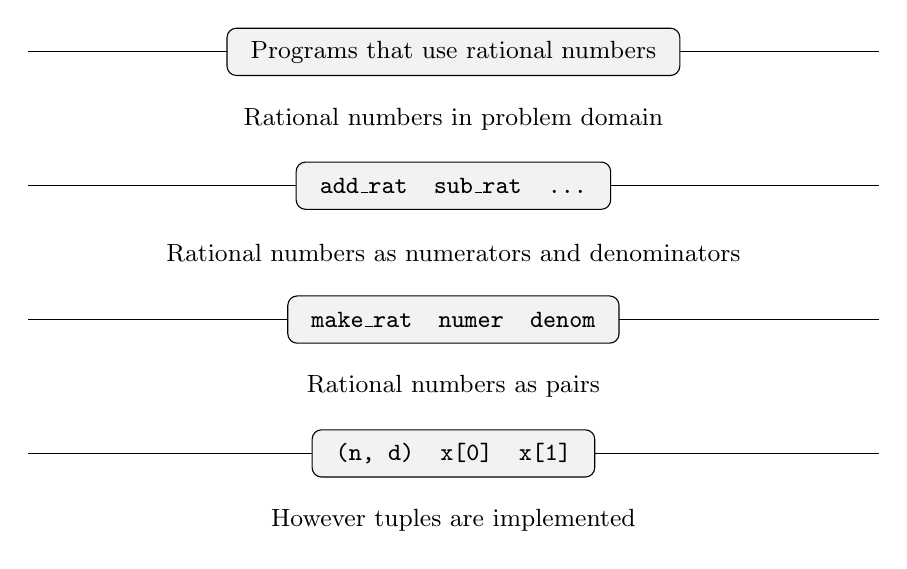
\begin{tikzpicture}[
  x = 1mm, y = 1mm,
  rule/.style = {draw, thin},
  box/.style  = {draw, thin, fill=black!5, rounded corners=1.2mm,
                 minimum height=6mm, inner xsep=3mm, font=\small},
  what/.style = {font=\small},
]

\def\halfwidth{54}

\foreach \y/\label in {%
    0/{Programs that use rational numbers},
    -17/{\ttfamily add\_rat\quad sub\_rat\quad \dots},
    -34/{\ttfamily make\_rat\quad numer\quad denom},
    -51/{\ttfamily (n, d)\quad x[0]\quad x[1]}%
  }{%
    \draw[rule] (-\halfwidth, \y) -- (\halfwidth, \y);
    \node[box] at (0, \y) {\label};
  }

\foreach \y/\label in {%
    -8.5/{Rational numbers in problem domain},
    -25.5/{Rational numbers as numerators and denominators},
    -42.5/{Rational numbers as pairs},
    -59.5/{However tuples are implemented}%
  }{%
    \node[what] at (0, \y) {\label};
  }

\end{tikzpicture}

\end{imageFigure}

We can envision the structure of the rational-number system as shown in
\link{Figure 2.1}.  The horizontal lines represent \newterm{abstraction
barriers} that isolate different ``levels'' of the system.  At each level, the
barrier separates the programs (above) that use the data abstraction from the
programs (below) that implement the data abstraction.  Programs that use
rational numbers manipulate them solely in terms of the procedures supplied
``for public use'' by the rational-number package: \code{add\_rat},
\code{sub\_rat}, \code{mul\_rat}, \code{div\_rat}, and \code{is\_equal\_rat}.
These, in turn, are implemented solely in terms of the constructor and selectors
\code{make\_rat}, \code{numer}, and \code{denom}, which themselves are
implemented in terms of pairs.  The details of how pairs are implemented are
irrelevant to the rest of the rational-number package so long as pairs can be
manipulated by writing a tuple and taking its parts out by position.  In
effect,
procedures at each level are the interfaces that define the abstraction
barriers and connect the different levels.

This simple idea has many advantages.  One advantage is that it makes programs
much easier to maintain and to modify.  Any complex data structure can be
represented in a variety of ways with the primitive data structures provided by
a programming language.  Of course, the choice of representation influences the
programs that operate on it; thus, if the representation were to be changed at
some later time, all such programs might have to be modified accordingly.  This
task could be time-consuming and expensive in the case of large programs unless
the dependence on the representation were to be confined by design to a very
few program modules.

For example, an alternate way to address the problem of reducing rational
numbers to lowest terms is to perform the reduction whenever we access the
parts of a rational number, rather than when we construct it.  This leads to
different constructor and selector procedures:

\begin{codeBlock}
>>> def make_rat(n, d):
...     return (n, d)

>>> def numer(x):
...     g = gcd(x[0], x[1])
...     return x[0] // g

>>> def denom(x):
...     g = gcd(x[0], x[1])
...     return x[1] // g
\end{codeBlock}

\noindent
The difference between this implementation and the previous one lies in when we
compute the \code{gcd}.  If in our typical use of rational numbers we access
the numerators and denominators of the same rational numbers many times, it
would be preferable to compute the \code{gcd} when the rational numbers are
constructed.  If not, we may be better off waiting until access time to compute
the \code{gcd}.  In any case, when we change from one representation to the
other, the procedures \code{add\_rat}, \code{sub\_rat}, and so on do not have to
be modified at all.

Constraining the dependence on the representation to a few interface procedures
helps us design programs as well as modify them, because it allows us to
maintain the flexibility to consider alternate implementations.  To continue
with our simple example, suppose we are designing a rational-number package and
we can't decide initially whether to perform the \code{gcd} at construction
time or at selection time.  The data-abstraction methodology gives us a way to
defer that decision without losing the ability to make progress on the rest of
the system.

\begin{exerciseGroup}
\phantomsection\label{Exercise 2.2}
\exerciseHeading{Exercise 2.2:} Consider the problem of
representing line segments in a plane.  Each segment is represented as a pair
of points: a starting point and an ending point.  Define a constructor
\code{make\_segment} and selectors \code{start\_segment} and \code{end\_segment}
that define the representation of segments in terms of points.  Furthermore, a
point can be represented as a pair of numbers: the \( x \) coordinate and the
\( y \) coordinate.  Accordingly, specify a constructor \code{make\_point} and
selectors \code{x\_point} and \code{y\_point} that define this representation.
Finally, using your selectors and constructors, define a procedure
\code{midpoint\_segment} that takes a line segment as argument and returns its
midpoint (the point whose coordinates are the average of the coordinates of the
endpoints).  To try your procedures, you'll need a way to print points:

\begin{codeBlock}
>>> def print_point(p):
...     print(f"({x_point(p)},{y_point(p)})")
\end{codeBlock}

\phantomsection\label{Exercise 2.3}
\exerciseHeading{Exercise 2.3:} Implement a representation for
rectangles in a plane.  (Hint: You may want to make use of \link{Exercise 2.2}.)
In terms of your constructors and selectors, create procedures that compute the
perimeter and the area of a given rectangle.  Now implement a different
representation for rectangles.  Can you design your system with suitable
abstraction barriers, so that the same perimeter and area procedures will work
using either representation?
\end{exerciseGroup}

